\documentclass[12pt, letterpaper]{article}
%\documentclass[12pt, letterpaper]{amsart}

%%%%%%%%%%%% LANGUAGE & ENCODING %%%%%%%%%%%%%%%%%
\usepackage[english]{babel}
\usepackage[utf8]{inputenc}%%%% to process umlauts and accents directly
%\usepackage{indentfirst}
%\usepackage{ucs}

%%%%%%%%%%% PACKAGES %%%%%%%%%%%%%%%%%%%%%%%%%%%%%
% For Hyperlinks
\usepackage[colorlinks,linkcolor=cyan,citecolor=magenta]{hyperref}

% Common math packages
\usepackage{amsthm, amsmath, amsfonts, amssymb, esint, mathrsfs, mathtools}
\usepackage{tensor} % To handle multi-index notation
\usepackage[capitalize,nameinlink]{cleveref} % Nice references
\crefname{equation}{}{} % Removes Eq. from equation references
\numberwithin{equation}{section} % Number equations within each section separately

% Extra symbols
\usepackage{stmaryrd} % contains \owedge  for Kulkarni-Nomizu product and some other special characters
\usepackage{commath} % contains \norm \abs

% Some useful packages
\usepackage{verbatim} %%% enables \begin{comment}    \end{comment}
\usepackage{enumerate} % allows different types of indices
\usepackage{float} % Handling figures

%%%%%%%%%%% MARGINS %%%%%%%%%%%%%%%%%%%%%%%%%%%%%%%%
% Margins
\usepackage[top=1in, bottom=1in, left=1in, right=1in]{geometry}

%%%%%%%%%%% CUSTOM NOTATION  %%%%%%%%%%%%%%%%%%%%%%
\newcommand{\N}{\mathbb{N}}
\newcommand{\Z}{\mathbb{Z}}
\newcommand{\Q}{\mathbb{Q}}
\newcommand{\R}{\mathbb{R}}
\newcommand{\C}{\mathbb{C}}
\newcommand{\K}{\mathbb{K}}

\newcommand{\f}{\mathfrak}
\newcommand{\ul}{\underline}
\newcommand{\mb}{\mathbb}
\newcommand{\mr}{\mathrm}
\newcommand{\mf}{\mathbf}
\newcommand{\mc}{\mathcal}
\newcommand{\e}{\emph}
\newcommand{\vp}{\varphi}
\newcommand{\ve}{\varepsilon}

\newcommand{\vol}{\operatorname{Vol}}
\newcommand{\diam}{\operatorname{diam}}
\newcommand{\dist}{\operatorname{dist}}
\newcommand{\dv}{\operatorname{div}}
\newcommand{\tr}{\operatorname{tr}}

\newcommand{\dd}{\; \mathrm{d}} %%%% d for integration dx
\newcommand{\wt}{\widetilde}
\newcommand{\ol}{\overline}

%%%%%%%%%%% THEOREMS %%%%%%%%%%%%%%%%%%%%%%%%
\newtheorem{theorem}{Theorem}[section]
\newtheorem{lemma}[theorem]{Lemma}
\newtheorem{proposition}[theorem]{Proposition}
\newtheorem{conjecture}[theorem]{Conjecture}
\newtheorem{corollary}[theorem]{Corollary}
\newtheorem{claim}[theorem]{Claim}
\newtheorem{problem}[theorem]{Problem}
\newtheorem{remark}[theorem]{Remark}

\theoremstyle{definition}
\newtheorem{definition}[theorem]{Definition}

\theoremstyle{remark}
\newtheorem{example}[theorem]{Example}


%%%%%%%%%%% TITLE %%%%%%%%%%%%%%%%%%%
%\title[CIS625: Computational Learning Theory]{Computational Learning Theory Lecture Notes}
%\author[Notes by Martin Citoler-Saumell]{Martin Citoler-Saumell}
%\date{Spring 2017}
%\address{University of Pennsylvania\\ Philadelphia, PA 19104}
%\email{\href{mailto:martinci@math.upenn.edu}{martinci@math.upenn.edu}}

\title{Computational Learning Theory Lecture Notes}
\author{Martin Citoler-Saumell}
\date{CIS625 Spring 2017}

%%%%%%%%%%% DOCUMENT BEGINS %%%%%%%%%%%%
\begin{document}

\maketitle

These are notes from \href{http://www.cis.upenn.edu/~mkearns/}{Prof. Michael Kearns}'s CIS625. 
This course is currently being taught at the University of Pennsylvania and attempts to provide algorithmic, complexity-theoretic and probabilistic foundations to modern machine learning and related topics.
 You can find out more at the \href{http://www.cis.upenn.edu/~mkearns/teaching/COLT/}{course website}. 
 A word of caution, it is likely that some typos and/or errors have been introduced during the taking of these notes. If you find any, please let me know at \href{mailto:martinci@math.upenn.edu}{martinci@math.upenn.edu}.

%------------------------------------------------------------
%          LECTURE 1
%------------------------------------------------------------
\section{Lecture 1: 2017.01.23}

\subsection{Course Outline/Description}

\subsubsection{Formal Models of ML}

\begin{itemize}
	\item Assumptions about data generation process.
	\item Assumptions about what algorithms "knows".
	\item Sources of info that the algorithms has
	\item Criteria/objective of learning is.
	\item Restrictions on algorithms.
\end{itemize}
	
\subsubsection{Examples of Models}

\begin{itemize}
	\item "PAC" model (in first 1/2 of the term).
	\item Statistical learning theory.
	\item "no-regrets" learning models.
	\item Reinforcement learning.
	\item ML \& Differential privacy.
	\item "Fairness" in ML
\end{itemize}


\subsection{A Rectangle Learning Problem}

Suppose you are trying to teach an alien friend the "shape" of humans in terms of abstract descriptions like "medium build", "athletic", etc. 
We are going to assume that each one of these descriptions represents a rectangular region on the height-weight plane but we are not aware of the exact dimensions. 
The only thing we are able to tell the alien is whether a particular individual is medium built or not. i.e. we can only label examples.

\begin{itemize}
	\item \ul{target} rectangle $R$, the \emph{true} notion of "medium built".
	\item \ul{hypothesis} rectangle $\hat R$. 
\end{itemize}

\begin{remark}
	Note that the assumption that the classifier function is a rectangle is rather strong. 
	There is always this trade-off to be able to actually compute things. 
	From a Bayesian point of view, ``we always need a prior''.
\end{remark}

Given a data cloud of examples, a reasonable hypothesis rectangle could be the tightest fit rectangle. 
However, this choice ignores the negative examples so it seems that that we are throwing away information. 
In a sense, this rectangle would be the least likely.

\begin{itemize}
	\item Assume $\langle x_1,x_2 \rangle$ pairs of height-weight are i.i.d. from an arbitrary unknown probability distribution, $D$.
\end{itemize}

We want to be able to evaluate how our hypothesis rectangle is performing. 
We want bounds on the classification error, which can be thought as the size of the symmetric difference between $R$ and $\hat R$
\begin{align}
	D[R\triangle \hat R] \equiv \mb P_D[R(\vec x) \ne \hat R(\vec x)].
\end{align}

\begin{theorem}
	Given $\ve,\delta >0$, there is some integer $N$ such that if we have more than $N$ training examples,\footnote{This the same as saying that sample size is at least $N$.} we have
	\begin{align}
		D[R\triangle \hat R] \equiv \mb P_D[R(\vec x) \ne \hat R(\vec x)] < \ve,
	\end{align}
	with probability at least $1-\delta$.
\end{theorem}

\begin{proof}
	First of all, note that using tightest fit, the hypothesis rectangle is always contained inside the target rectangle. 
	Now, for each side of the target rectangle we may draw inward strips in such a way that each strip has $\mb P_D[Strip] < \frac{\ve}{4}$. 
	If the training set has a positive example in each of these four strips, then the inequality above is satisfied because the boundary of the hypothesis rectangle would be contained in the union of the strips. 
	Next we need to deal with the required sample size to obtain this result with some certainty. 
	Let $m$ denote the sample size, since the distribution is i.i.d., we have
	\begin{align*}
		\mb P_D[\textrm{miss a specific strip m times}] = \left(1-\frac{\ve}{4}\right)^m,\\
		\mb P_D[\textrm{miss any of the strips m times}] \geq 4\left(1-\frac{\ve}{4}\right)^m.
	\end{align*}
	By the discussion above, the last inequality implies
	\begin{align*}
		\mb P_{D^m}[D[R\triangle\hat R]\geq \ve] \leq 4\left(1-\frac{\ve}{4}\right)^m,
	\end{align*}
	which can be chosen arbitrarily small for big enough $m$. 
	One can obtain $N\geq \frac4\ve \ln\left(\frac4\delta\right)$.
\end{proof}

\begin{remark}
	This proof generalizes to $d$-dimensional rectangles. 
	We only need to replace 4 with $2d$, the number of $(d-1)$-faces.
	We can also try to incorporate noisy data, where the labels have some probability of being wrong.
\end{remark}


\subsection{A More General Model}

\begin{itemize}
	\item Input/instance/feature space, $X$. (e.g. $\R^2$ in the example above)
	\item Concept/classifier/boolean function, $C: X \rightarrow \left\{0,1\right\}$ or we can also think about it as an indicator function of the positive examples or the subset of positive examples.
	\item Concept class/target class, $\mc C \subset \mc P(X)$, the admissible concepts/classifiers. (e.g. all rectangles in $\R^2$ in the example above)
	\item \ul{target} concept, $c\in\mc C$. (e.g. target rectangle in the example above)
	\item Input distribution, $D$ over $X$ (arbitrary \& unknown)
	\item Learning algorithm given access to examples of the form: $\langle \vec x,y \rangle$ where $\vec x$ is i.i.d. drawn from $D$ and $c(\vec x) = y$.
\end{itemize}

\begin{definition}[PAC Learning]
	We say that a class of functions over $X$, $\mc C$, is \emph{Probably Approximately Correct (PAC) learnable} if there exists an algorithm, $L$, such that given any $c$ in $\mc C$, $D$ a distribution over $X$ and $\ve, \delta >0$, $L$ with these parameters and random inputs $\vec x$'s satisfies:  
	\begin{itemize}
		\item (Learning) With probability $\geq 1 -\delta$, $L$ outputs a hypothesis, $h$ in $\mc 
		C$ such that $D[h\triangle c]<\ve$, i. e.
		\begin{align}
    		Err(h) \coloneqq \mb P_{x\sim D}[h(x) \ne c(x)] \leq \ve.
		\end{align}
		\item (Efficient) $L$ runs in time/sample $poly\left(\frac1\ve, \frac1\delta, \textrm{dimension}\right)$.
	\end{itemize}
\end{definition}


%------------------------------------------------------------
%          LECTURE 2
%------------------------------------------------------------
\section{Lecture 2: 2017.01.30}

\begin{remark}[PAC Learning]
    Fixing the class $\mc C$ is a strong assumption, it is the prior you are assuming about the true behavior of the data.
     For example, when you fit a linear regression, you are assuming that there is a true linear relation in the data.
    
    In contrast, the assumption on the distribution over $X$ is fairly general.
\end{remark}

\begin{theorem}
    The class of rectangles over $\R^2$ from example above is PAC learnable (with sample size $m\sim\frac1\ve\ln\left(\frac1\delta\right)$).
\end{theorem}

\subsection{PAC learning boolean conjunctions}

In the following we are going to see an example of problem that is PAC learnable.
\begin{itemize}
    \item $X = \lbrace 0, 1 \rbrace^n$
    \item Class $\mc C = $ all conjunctions over $x_1,\ldots,x_n$. $\abs{\mc C} = 3^n$\\
          E.g.: If $c = x_1\wedge \lnot x_3 \wedge \lnot x_{11} \wedge x_{26} \ldots$,
          \begin{align}
              c(\vec x) = 1 \iff x_1 =1, x_3 = 0, x_{11} = 0, x_{26} = 1, \ldots
          \end{align}
    \item $D$ over $\lbrace 0, 1 \rbrace^n$.
\end{itemize}


\subsubsection[Algorithm for monotone case]{Algorithm for monotone case (i.e. no $\lnot$'s)}

In this case we are trying to fit something like $c = x_1\wedge x_5 \wedge x_{13} \ldots$. i.e. given some examples of sequences of bits and the result of $c$ on them, we are trying to guess what the conjunction $c$ actually is.
We can use the following algorithm:
\begin{itemize}
    \item $h \leftarrow x_1\wedge x_2 \wedge x_3\wedge \ldots \wedge x_n$, start with the conjunction of all the variables.
    \item For each positive example, $\langle \vec x, 1 \rangle$, delete any variable in $h$ such that $x_i=0$.\\
    This method ensures that the positives of $h$ is a subset of the true $c$.
\end{itemize}


\subsubsection*{Analysis}

Let $p_i$ denote the probability we delete $x_i$ from $h$ in a single draw. In other words,
\begin{align}
    p_i = \mb P_{\bar X\sim D}[c(\vec x) = 1, x_i=0].
\end{align}
Then we have an a priori bound on error: $Err(h) \leq \sum\limits_{x_i\in h} p_i$.
 We can make a distinction between \emph{bad} and \emph{good} indices. 
 An index, $i$, is bad if $p_i\geq \frac{\ve}{n}$ and good otherwise. 
 Note that if $h$ contains no bad indices, then we have
\begin{align}
    Err(h) \leq \sum\limits_{x_i\in h} p_i \leq n\left(\frac{\ve}{n}\right).
\end{align}
Let's fix some index, $i$, such that $p_i\geq \frac\ve n$. i.e. a bad index. We have that
\begin{align}
    \mb P[x_i\textrm{ "survives" m random samples}] &= (1 - p_i)^m \quad (iid)\\
    & \leq \left(1 - \frac\ve n\right)^m \\
    \mb P[\textrm{\emph{any} bad i "survives" m random samples}] &\leq n\left(1 - \frac\ve n\right)^m.
\end{align}
If we want the right-hand-side of the last inequality to be less than some $\delta>0$, we end up with $m \geq \frac n\ve \ln\left(\frac n\delta\right)$. 
In other words, we just proved the following theorem

\begin{theorem}
    Conjunctions over $\lbrace 0,1 \rbrace^n$ are PAC learnable with sample size  $m \geq \frac n\ve \ln\left(\frac n\delta\right)$.
\end{theorem}

\begin{remark}
    An analogous argument proves this theorem for conjunctions that are not necessarily monotone. 
    The only difference is that we have to keep track the extra $\lnot$ variables.
\end{remark}

\begin{remark}
    We can identify some pattern for this kind of analysis. 
    We identify some ``bad'' things that may happen and then prove that the probability of them happening decreases fast when we increase the number of samples seen.
\end{remark}


\subsection{Hardness of PAC learning 3-term DNF}

Now we are going to see an example of non PAC learnable problem. 
However, we will be able to slightly modify it and achieve PAC learning. 
This motivates an better definition of PAC learnable.
\begin{itemize}
    \item Input space $X = \lbrace 0, 1 \rbrace^n$
    \item Class $\mc C = $ all disjunctions of three conjunctions. $\abs{\mc C} = 3^{3n}$\\
          E.g.: If $c = T_1 \lor T_2 \lor T_3$ where $T_i$ is a conjunction over $X$.\\
          $c = \left(x_1 \wedge x_7 \wedge \lnot x_8 \right) \lor \left(x_2 \wedge x_5 \wedge \lnot x_7 \wedge \lnot x_8\right) \lor \left(x_6 \wedge x_{12}\right)$.
\end{itemize}
To see that this problem is \emph{hard}, we prove that the graph 3-coloring problem reduces to the 3-term DNF problem. 

\subsubsection*{Graph 3-coloring to PAC learning 3-term DNF}

Suppose that you have a 3-colorable (undirected) graph $G$. 
That is, a graph such that we can color the vertices with 3 colors in such a way that there are no edges between vertices of the same color. 
We see an example of how to transform such a graph into a set of labeled examples for the PAC learning 3-term DNF. 
\begin{figure}[H]
\centering
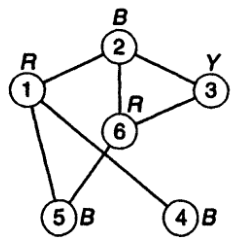
\includegraphics[width=0.3\linewidth]{img/graph}
\caption{A graph with a 3-coloring.}
\label{fig:graph}
\end{figure}
First, for the $i$-th node we create a positive example that is represented by the vector, $v(i)$, with a 0 in the $i$-th entry and 1's everywhere else. E.g. from node one we have $\langle 011111, + \rangle$.
Then we create a negative example from each edge that is represented by a vector, $e(i,j)$, of 1's except for 0's at the positions that determine the edge. 
E.g. from the edge connecting 2 and 3 we obtain $\langle 100111, - \rangle$.
Next, the coloring can be used to define a 3-term DNF in the following way. 
Given a color, we define $T_{color}$ as the conjunction of the variables/vertices that are \emph{not} of that color. In this example we have
\begin{align}
    T_R = x_2 \wedge x_3 \wedge x_4 \wedge x_5,\\
    T_B = x_1 \wedge x_3 \wedge x_6,\\
    T_Y = x_1 \wedge x_2 \wedge x_4 \land x_5 \land x_6 .
\end{align}

\begin{claim}
    $G$ is 3-colorable $\iff$ there is a 3-term DNF \emph{consistent} with the labeled sample above.
\end{claim}
\begin{proof}
    We have just seen how to obtain a 3-term DNF from a 3-colorable graph. We only need to check that it is consistent with the sample. 
    By construction, all the positive examples satisfy $T_{color}$ where color is the vertex's color, since the only 0 in the vector is in the position that is dropped. 
    Similarly, it follows that the examples coming from the edges do not satisfy any of the $T$'s. In any edge there are two colors corresponding to its vertices. 
    The extra 0 in the example ensures that the $T$'s from those colors are not satisfied.
    Finally, the $T$ of the remaining color cannot be satisfied because both vertices are included in the conjunction and they are both 0 in the example.
    
    Conversely, given a graph and the labeled examples as above, if there is a consistent 3-term DNF we can find a coloring in the following way. 
    Label each term of the formula with a color, say $T_R \lor T_Y \lor T_B$, and remember the order of the labels. 
    Then, we define the color of vertex $i$ (corresponding to vector $1\ldots101\ldots1$) as the label of the first formula that is satisfied by $v(i)$. 
    Since the formula is consistent with the sample, every vertex must be actually colored. We only need to argue that this is a valid coloring. 
    Suppose to the contrary that $i$ and $j$ are to vertices that are connected by an edge and have the same color. 
    This means that both $v(i)$ and $v(j)$ satisfy $T_{C_0}$. 
    However, we also have $v(i) \& v(j) = e(i,j)$  where $\&$ denotes the bit-wise and operation and it follows that $e(i,j)$ satisfies $T_{C_0}$, a contradiction with the consistency of the formula since edges are negative examples.
\end{proof}

This concludes the argument that finding a coloring of a graph is the same as producing a consistent 3-term DNF. 
We are only left with the computational aspects.
Namely, given the labeled sample associated to a graph, we need to find a way to feed it to a PAC learning algorithm. 
First we need a distribution over vectors of bits.
For this we can just sample the examples uniformly. 
Finally, to ensure consistency we choose $\ve$ any quantity less than $\frac1{\#examples}$\footnote{This epsilon is allowed because $\frac1\ve$ is polynomial in the size of input. This is not true in general.}. This way the algorithm cannot make any mistakes is forced to be consistent. The $\delta$ can be arbitrary.
In conclusion, if the 3-term DNF problem were PAC learnable, we could solve the coloring problem in random polynomial time. 
Another way to say this is in the form of the following theorem.
\begin{theorem}
    If 3-term DNF are PAC learnable, then $NP = RP$.
\end{theorem}
Of course, it is strongly believed that $RP \subsetneq NP$ so this is rather strong evidence against the easiness of the 3-term DNF problem.

\begin{remark}
    The upshot is that a slight generalization of the conjunction problem, for which we have a randomized polynomial time solution, is almost assured to not be PAC learnable ( unless NP = RP)
\end{remark}




%------------------------------------------------------------
%          LECTURE 3
%------------------------------------------------------------
\section{Lecture 3: 2017.02.06}

Recall the definition of a class being PAC learnable.
\begin{definition}[PAC Learning]
	A class $\mc C$ is \emph{Probably Approximately Correct (PAC) learnable} if there exists an algorithm, $L$, such that:
	\begin{align}
    	\forall c \in \mc C,\quad \forall D \textrm{ over }X,\quad \forall \ve,\delta > 0
	\end{align} 
	\begin{itemize}
		\item (Learning) With probability $\geq 1 -\delta$, $L$ outputs a hypothesis, $h$ in $\mc 
		C$ such that $D[h\triangle c]<\ve$, i.e. we have error at most $\ve$
		\begin{align}
    		Err(h) \coloneqq \mb P_{x\sim D}[h(x) \ne c(x)] \leq \ve.
		\end{align}
		\item (Efficient) $L$ runs in time/sample $poly\left(\frac1\ve, \frac1\delta, n\right)$. \emph{Samples} \& \emph{computation}.
	\end{itemize}
\end{definition}
\begin{remark}
    Usually when we talk about computation time we are in the realm of complexity theory and we talk about samples we are really asking statistics/information-theory questions about what sample size do we need to be able to draw some conclusion.
\end{remark}

\subsection{PAC learning 3-term DNF by 3-CNF}
In the following we see how to overcome the intractability of the 3-DNF PAC learning by using a different representation. It amounts to expanding the input space and the class we are learning.

\begin{definition}
    A 3-CNF is a conjunction of disjunctions of length three.
\end{definition}

Given a 3-DNF, we can rewrite it as a 3-CNF in the following way:
\begin{align}
    T_1 \lor T_2 \lor T_3 \equiv \bigwedge\limits_{\stackrel{u\in T_1}{\stackrel{v\in T_2}{w\in T_3}}} \left(u \lor v \lor w\right),
\end{align}
for every assignment of $x_1,\ldots,x_n$, both sides evaluate to the same boolean value. Notice that the length of the 3-CNF can be much bigger (but still polynomial): 3-DNF is at most as $3n$ but 3-CNF could be up to $n^3$. In a sense, this corresponds to feature generation.
\begin{remark}
    Notice that the reverse is NOT true. Given a 3-CNF it might not be representable as a 3-DNF. 
    
    Another important point to notice is that after the transformation into 3-CNF we are changing the distribution of the initial input space. But the definition of PAC learnable allows for \emph{any} distribution, so we are fine.
\end{remark}

The upshot here is that we can learn 3-CNF by 3-CNF but this problem contains the intractable problem of learning 3-DNF by 3-DNF. The trick is that we have a bigger solution space so we the 3-CNF algorithm is fed a 3-DNF, it has the option to output something outside the 3-DNF class, namely a 3-CNF.

\begin{theorem}
    3-CNF is PAC-learnable and 3-DNF. Further, by the discussion above, 3-DNF is learnable ``by'' 3-CNF.
\end{theorem}

This motivates the more general definition for PAC-learnable that takes into account the solution class.
\begin{definition}[PAC Learning]
	A class $\mc C$ is \emph{Probably Approximately Correct (PAC) learnable} by $\mc C \subset \mc H$ if there exists an algorithm, $L$, such that:
	\begin{align}
    	\forall c \in \mc C,\quad \forall D \textrm{ over }X,\quad \forall \ve,\delta > 0
	\end{align} 
	\begin{itemize}
		\item (Learning) With probability $\geq 1 -\delta$, $L$ outputs a hypothesis, $\ul{h\in\mc H}$ 
		 such that $D[h\triangle c]<\ve$, i.e. we have error at most $\ve$
		\begin{align}
    		Err(h) \coloneqq \mb P_{x\sim D}[h(x) \ne c(x)] \leq \ve.
		\end{align}
		\item (Efficient) $L$ runs in time/sample $poly\left(\frac1\ve, \frac1\delta, n\right)$. \emph{Samples} \& \emph{computation}.
	\end{itemize}
\end{definition}
\begin{remark}
     $\mc C$ is usually called the target class and $\mc H$ the hypothesis class.
\end{remark}


\subsection{Consistency implies PAC-learnable}
\begin{itemize}
\item Suppose we have some target and hypothesis classes, $\mc C \subset \mc H$.
\item Let $A$ be a \emph{consistent} algorithm:
    \begin{enumerate}[i)]
    \item Given \ul{any} finite sample, $S=\lbrace \langle x_1,y_1\rangle,\ldots,\langle x_m,y_m\rangle\rbrace$, where  for all $i$ we have $y_i = c(x_i)$ for some $c\in \mc C$.
    \item $A$ outputs $h\in\mc H$ such that $h(x_i)=y_i=c(x_i)$ for all $i$.
    \end{enumerate}
\end{itemize}

\begin{theorem}
    For any finite $\mc H$, a  consistent algorithm  for $\mc H$ is a PAC-learnable algorithm.
\end{theorem}
\begin{proof}
    We call a hypothesis, $h\in\mc H$, $\ve$-bad if $Err(h)>\ve$. Now we generate a size-$m$ $S$ according to $Ex(c, D)$, which is the subroutine that generates samples from $D$. For any \ul{fixed} $\ve$-bad $h$, we have an upper bound on the probability of $h$ being consistent with $S$
    \begin{align}
        \mb P_{S}[h\textrm{ consistent with }S] \leq (1-\ve)^m.
    \end{align}
    Therefore,  $\mb P_{S}[\exists h\in\mc H\textrm{ that is both $\ve$-bad and consistent with } S] \leq \abs{\mc H}(1-\ve)^m$. Now we choose $\delta > 0$ such that  $\abs{\mc H}(1-\ve)^m < \delta$. We can conclude that as long as $m \geq \frac{const}\ve \ln\frac{\abs{\mc H}}\delta$ the PAC learning definition will be satisfied.
\end{proof}
\begin{remark}
    $\abs{\mc H}(1-\ve)^m \leq e^{ \ln\abs{\mc H} + m\ln(1-\ve)}\approx e^{\ln\abs{\mc H} - c_0\ve m} \to 0$ as $m\to\infty$. A key point of this is that we can let the complexity of the hypothesis to grow as the sample size gets bigger and keeping this quantity under control. That is, the more data you have, the more complex the model you can train without over-fitting too much. If $\mc H_m$ is the hypothesis for data of size $m$, we only need $\ln\abs{\mc H_m} \leq c \cdot m^\beta$, for some $\beta < 1$ and $c=c(dim)$. From here we obtain $ m \geq \left(\frac c\ve\right)^{\frac1{1-\beta}}$.
\end{remark}

Next we want to deal with the case of a possibly infinite hypothesis class $\mc H$. The first approach could be to try and force feed a discretization of the hypothesis into the finite case one but this might not work because it depends on the interaction between the distribution of the data and the chosen discretization. We want something better.

\begin{itemize}
    \item Class $\mc H$ over $X$.
    \item $h\in \mc H$ as functions $h(x)\in \lbrace0,1\rbrace$; or as sets $h\subset X$.
    \item Let $S=\lbrace x_1,\ldots,x_m\rbrace$ be an \ul{ordered} subset of $X$.
    \item $\Pi_{\mc H}(S) = \left\{\langle h(x_1),\ldots,h(x_n)\rangle:h\in\mc H\right\} \subseteq \lbrace0,1\rbrace^m$
    \begin{remark}
        If the inclusion above is saturated then it means that our hypothesis can classify ANY labeling of that size. That is bad for learning because it is saying that there is no structure in the data.
    \end{remark}
    \item {\bf [Definition]} We say that $S$ is \emph{shattered} if the the equality case holds, $\Pi_{\mc H}(S) = \lbrace 0, 1\rbrace^m$, or equivalently, $\abs{\Pi_{\mc H}(S)} = 2^m$.
    \item {\bf [Definition]} The Vapnik-Chervonenkis dimension of $\mc H$ as
            \begin{align}
                VCD(\mc H) &= \textrm{ size of the \ul{largest} shattered set}\\
                             &= \max\limits_d\left\{\exists S\subseteq X:\;\abs{S}=d\quad\&\quad\Pi_{\mc H}(S) = \lbrace 0,1\rbrace^d\right\}
            \end{align}
    \paragraph{Example.} If $\mc H$ is finite, then $VCD(\mc C)\leq \ln\abs{\mc C}$ because shattered $d$ points requires $2^d$ functions.
    
    \paragraph{Rectangles in $\R^2$.} The VCD dimension is $4$ in this case because the rectangular convex hull of a set of points is always given by the four extremal points in each direction.
\end{itemize}
\end{document}
